\documentclass[]{report}
\usepackage{graphicx}
\usepackage{todonotes}	
\usepackage{booktabs}
\usepackage{listings}
\usepackage[margin=1in]{geometry}

\graphicspath{{resources/images/}}



% Title Page
\title{Utilising peer-to-peer networking for data transfer over the browser}
\author{Dominic Rathbone}


\begin{document}
\maketitle
\tableofcontents
\listoftodos

\chapter{Interim Planning \& Investigation Report}
	\section{Project Scope}
		\subsection*{Aims and Objectives}
			The ultimate objective of my project is to investigate the possibility of data transfer over web browsers (in particular audio and video streaming) without the need for a centralised client-server architecture, instead opting for a peer-to-peer network architecture. In order to do so, I plan to:
			\begin{itemize}
				\item Research peer-to-peer networking architecture
				\item Research WebRTC
				\item Research signalling protocols
				\item Research media streaming compression \& protocols
				\item Research client-side JavaScript frameworks
				\item Develop a session signalling server in Java with the WebSockets protocol
				\item Develop a WebRTC Application to transfer and stream uploaded files.
				\item Implement a peer to peer network between peers transfering/streaming a file using the web application.
			\end{itemize}
		\subsection*{Stakeholders}
			The stakeholders involved in my project will be myself, my supervisor, Stelios Kapetanakis and the user.
		\subsection*{Methods of Communication}
			Stelios and I have set up a regular meeting once a week on Friday at 4pm to review progress and answer any questions. On top of this, we communicate regularly via email and Stelios has access to a project git repository on GitHub and a workflow board set up on my web server to monitor the progress of my project. 
			
	\section{Research}
		\subsection*{Comparing Network Architectures}	
			Peer-to-peer networking is the distribution of resources and processing between the nodes of a network. These networks tend to take the form of an overlay network. An overlay network is a topology describing a virtual network that sits on top of a physical network (e.g the internet) consisting of a subset of the nodes connected to the physical network. 
			
			\begin{figure}[h]
				\caption{
					An Unstructured Peer-To-Peer Overlay Network 	
					\cite{Unstructured P2P Diagram}
				}
				\centering
				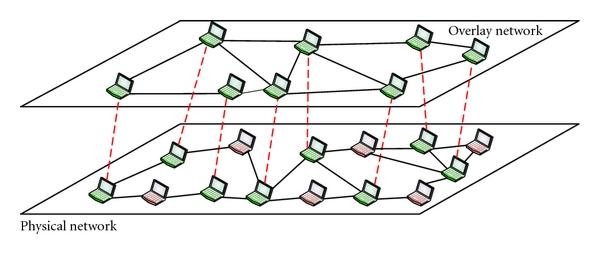
\includegraphics{overlaynetwork.jpg}
			\end{figure}
			
			Although an overlay network does not need to manage the burden the physical network is responsible for, in order to discover new nodes and route them together, it needs to have some way of managing this subset of nodes. This is normally achieved in 3 different ways:
			
			\begin{itemize}
				\item Unstructured peer-to-peer:
				Peer connections in the overlay are established randomly. New peers copy the connections another peer has formed and develops it's own over time. \cite{P2P overlay networks}
				\item Structured peer-to-peer:
				Peers in a network are organised using a distributed hash table (DHT). The DHT consists of many peers maintaining a partial hash table containing the unique keys of it's neighbouring peers, allowing it to route to them. This way, a node can communicate with another by hopping a message through other nodes until it is reached. \cite{P2P overlay networks}
				\item Hybrid peer-to-peer:
				A combination of  peer to peer and client-server models, peers are discovered and routed by a centralized signalling server. The responsibilities of this server can vary in degree as they can leave features that function better in decentralized networks to the nodes in order to improve performance whilst maintaing responsbility for the features that function better using a centralized server.\cite{Hybrid P2P network}
			\end{itemize}
			
			Currently, the most common network architecture for file storage/transfer and video streaming services is the client-server model. In a basic sense, this is when the machines processing data (servers) are distinct from the computers requesting this processing (client), although in actuality, the boundaries between the two split dependent on how it is implemented. Whilst the shift of processing on to the service supplier means that the user of the application does not need a powerful machine to run it, it also means that the service supplier has the responsibility of maintaining and paying for these servers. Furthermore, although modern server architectures are designed in a distributed structure granting them to be more robust (as distribution allows for redundancy and load balancing), if these servers undergo too much load or in extreme cases, if the server farm completely crashes, the user would not be able to use the application as intended.
			
			Using peer to peer architecture avoids these issues with the client-server model as processing is distributed between the nodes making up the network, resulting in it being cheaper to maintain and scale the service as load increases whilst being inherently robust. However, there are a number of considerations to be aware of in peer to peer networking. Security is a concern within peer-to-peer networking as there is no centralized authority to manage access control to resources. Thus, a malicious client could potentially launch a number of attacks versus other nodes in the network such as Denial Of Service (DoS) where a malicious group of nodes floods a network with a massive amount of fake data, potentially crashing nodes within it or Man in the Middle (MitM) attacks where a node is able to intercept data flowing between two other nodes and spy on or poison this data.\cite{P2P Security Issues}
			
			Whilst it would be hard to completely avoid risks like this as it is an inherent flaw in peer-to-peer architecture, introducing the basic concept of trust into a peer-to-peer network can stop malicious peers from entering it in the first place. Trust will be implemented in my application by allowing users to enable authentication (via password) for the uploaded file giving them a level of access control that would prevent malicious attackers from being able to join the network of peers involved in the download or stream of the file. 
	
		\subsection*{Current Solutions to Data Transfer}
			
			Currently, solutions such as DropBox and Google Drive focus on cloud storage as a service whilst providing the ability to transfer your data as a secondary function of this service. Although this is an extremely valuable and convenient idea enabling consumers to back-up their data, not all want a service that stores the data they want to transfer as the practice of storing data in the cloud does raise ethical issues, namely with it's security, privacy and ownership once it has been uploaded. However, this can be hard to avoid when the online storage and transfer of data are so closely intertwined.
			
			Once you have uploaded files to one of these services, there is a trust placed on the company to store the data securely. However, The "Cloud Security Alliance" released a regularly updated list of the top threats faced by cloud computing services in 2010 submitting there are numerous security issues faced within the cloud computing industry with many of the issues on this list occurring due to malicious intentions, for example the 6th item on the list, "malicious insiders" describes a situation in which current or former employees abuse their authorizations within system to gain access to sensitive information \cite{CSA Top Threats}. This suggests that even though companies can protect their client's data to an extent, there are still issues the industry face that consumers may want to avoid.
		 
		 	Whilst the uploaded data can be encrypted in a way that means only clients of the service can decrypt it (through end-to-end encryption), many people feel insecure leaving traces of their private information on a remote server belonging to a company that is not necessarily always acting in their interest. In 2013, this concern was legitimized by Edward Snowden when he disclosed information about government surveillance programs such as PRISM which coerced firms such as Google, Microsoft and Yahoo to provide private consumer data from their services to the government.\cite{PRISM}  More recently, this idea has been reinforced by legislation such as the "Investigatory Powers Bill" being introduced in the UK that could prohibit companies from using end-to-end encryption techniques allowing the government to request decrypted client data \cite{IPB Encryption}. Whilst we can assume the UK government have done this with non-malicious intentions, by weakening the encryption practices of these companies, they will potentially weaken the defence against malicious attackers.
			
			As an alternative to using cloud storage solutions for sharing files, there is also specific file sharing sites such as WeTransfer that allows you to send files up to 2gb via their site. This works by sending a link through email to the person you want to send the file to. Whilst it does store the uploaded files, they are only kept for 7 days in order to prevent unnecessary storage usage \cite{WeTransfer Storage Time}. Although this is better for data privacy, WeTransfer use third party providers such as Amazon Web Services (AWS) to store this data using AWS S3 Storage \cite{WeTransfer AWS Case Study} meaning there is still the potential concern of data privacy and security highlighted previously.
			
			Peer-to-peer networks have been also been popular for file sharing since the late 1990s due to the rise of applications such as Napster which allowed users to share music over one. Napster worked by using a central server to index files that each peer's made available on their machine. Each peer would then be able to search the index for copies of songs. However, this service was eventually shut down as the company ran into legal problems with copyright infringement. Since then, protocols such as BitTorrent have improved on the idea of peer to peer sharing. The BitTorrent protocol works by peers creating ".torrent" descriptor files that describe the file's metadata, this is then shared however it is seen fit. Each peer wanting to download this file then picks up this ".torrent" file, opens it with a BitTorrent client and becomes one of the many "leechers" trying to download this file. At the same time, this peer becomes one of the many "seeders" uploading this file as they download it so that other leechers can download it from them. The initial peer discovery is based on "trackers" which are servers hosting lists of seeders and leechers for the file. One of the issues with BitTorrent is that in order to share a file, you must go through the process of download a client, creating a ".torrent" file, add it to a trackers list and share the ".torrent" with the peers you wish to share it with and this can be seen as a arduous task for a basic consumer looking to share their files. 

			As an alternative to these current solutions, the application I plan to develop has the aim of separating the online transfer of data from it's storage by connecting the peers involved in the transfer directly with each other. This circumvents the problems with cloud storage as the data being transferred does not pass through any servers as well as the problems with current peer to peer file sharing as it does not require a desktop client or torrent files. To allow my application to share files online, WebRTC will be used.
			
			WebRTC (Real Time Communication) is an emerging web technology that enables browsers to communicate real time via a peer-to-peer connection, avoiding the need for a centralized server to transfer data between clients. This was first released by Google as an open source project in May 2011 \cite{Google WebRTC Release} and was later drafted as an API definition by W3C which is still a work in progress. \cite{W3C WebRTC Definition}. WebRTC has yet to be fully implemented in every web browser but Chrome, Firefox and a WebRTC specific browser called Bowser are leading the way in implementing the API definition. Firefox (Nightly) is leading the way in this so the application will specifically be developed towards this browser\cite{WebRTC browser support}.
			The 3 main WebRTC APIs supported at this time are:
				\begin{itemize}
					\item RTCDataChannel:
					"The RTCDataChannel interface represents a bi-directional data channel between two peers of a connection." \cite{Mozilla Web API}
					\item RTCPeerConnection:
					"The RTCPeerConnection interface represents a WebRTC connection between the local computer and a remote peer. It is used to handle efficient streaming of data between the two peers." 
					\cite{Mozilla Web API}
					\item getUserMedia:
					"Prompts the user for permission to use one video and/or one audio input device such as a camera or screensharing and/or a microphone. If the user provides permission, then the successCallback is invoked with the resulting MediaStream object as its argument. If the user denies permission or media is not available, then the errorCallback is called with PermissionDeniedError or NotFoundError respectively. Note that it is possible for neither completion callback to be called, as the user is not required to make a choice."
					\cite{Mozilla Web API}
				\end{itemize}

			In order to achieve it's aim, the application will utilize the RTCPeerConnection and RTCDataChannel APIs. The former to establish a peer connection between two clients and the latter to create a data channel over this peer connection to transfer data.	
			
			As mentioned in Javascript Session Establishment Protocol (JSEP)\cite{JSEP}, although WebRTC and the browser is used to transfer the data between two peers, it purposely does not handle signalling. Signalling is a concept that came from telecommunications and VoIP and is the process of organising the communication between two clients, handling the exchange of metadata that creates and manages a session. The rationale behind webRTC being protocol-agnostic with signalling is that different applications may require different protocols in order to, for example, fit into previously existing architecture. To handle signalling for my implementation of WebRTC, Session Initiation Protocol (SIP) over WebSockets will be used.
			
			\begin{figure}[h!]
				\caption{WebRTC Architecture as defined by JSEP \cite{JSEP}}
				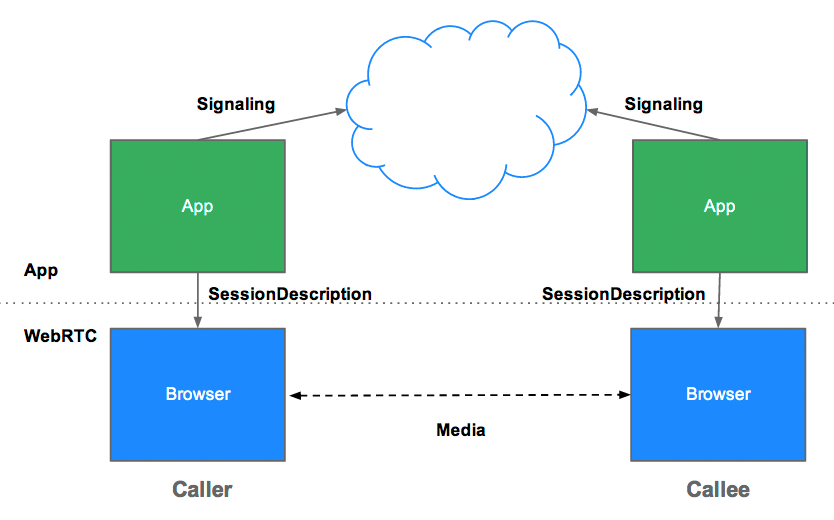
\includegraphics[scale=0.4]{jsep.png}
			\end{figure}
			\newpage
			
			WebSockets is a protocol implemented by browsers and web servers running over TCP to provide bi-directional communication between them. Once it establishes a session with a client connecting to the server, this session is left open for the server to send messages to the client and vice versa, making it a good candidate for signalling with a WebRTC application which needs peers to be able to reliably signal messages back and forth through the server. SIP is a communication protocol that does not specify how signals are transported (e.g WebSockets) but how these signals are defined. The transaction model defined by SIP is similar to HTTP with each SIP request being matched by a response.
			
			\subsubsection*{SIP Example}
			
			 Initial handshake with WebSocket signalling server over HTTP \\
			 dom -\textgreater\ sip.transfer4.me
			 \begin{lstlisting}[tabsize=1,frame=single, basicstyle=\ttfamily\footnotesize]
			 GET / HTTP/1.1
			 Host: proxy.example.com
			 Upgrade: websocket
			 Connection: Upgrade
			 Sec-WebSocket-Key: dGhlIHNhbXBsZSBub25jZQ==
			 Origin: https://www.example.com
			 Sec-WebSocket-Protocol: sip
			 Sec-WebSocket-Version: 13
			 \end{lstlisting}
			 Switching to WebSocket protocol \\
			 sip.transfer4.me -\textgreater\ dom
			 \begin{lstlisting}[tabsize=1,frame=single, basicstyle=\ttfamily\footnotesize]
			 HTTP/1.1 101 Switching Protocols
			 Upgrade: websocket
			 Connection: Upgrade
			 Sec-WebSocket-Accept: s3pPLMBiTxaQ9kYGzzhZRbK+xOo=
			 Sec-WebSocket-Protocol: sip
			 \end{lstlisting}
			 SIP REGISTER request letting the server know of Dom's "location" \\
			 dom -\textgreater\ sip.transfer4.me
			 \begin{lstlisting}[tabsize=1,frame=single, basicstyle=\ttfamily\footnotesize]
			 REGISTER sip:proxy.example.com SIP/2.0
			 Via: SIP/2.0/WSS df7jal23ls0d.invalid;branch=z9hG4bKasudf
			 From: sip:dom@example.com;tag=65bnmj.34asd
			 To: sip:dom@example.com
			 Call-ID: aiuy7k9njasd
			 CSeq: 1 REGISTER
			 Max-Forwards: 70
			 Supported: path, outbound, gruu
			 Contact: <sip:dom@df7jal23ls0d.invalid;transport=ws>
			 ;reg-id=1
			 ;+sip.instance="<urn:uuid:f81-7dec-14a06cf1>"
			 \end{lstlisting}
			 OK response \\
			 sip.transfer4.me -\textgreater\ Dom
			 \begin{lstlisting}[tabsize=1,frame=single, basicstyle=\ttfamily\footnotesize]
			 SIP/2.0 200 OK
			 Via: SIP/2.0/WSS df7jal23ls0d.invalid;branch=z9hG4bKasudf
			 From: sip:dom@example.com;tag=65bnmj.34asd
			 To: sip:dom@example.com;tag=12isjljn8
			 Call-ID: aiuy7k9njasd
			 CSeq: 1 REGISTER
			 Supported: outbound, gruu
			 Contact: <sip:alice@df7jal23ls0d.invalid;transport=ws>
			 ;reg-id=1
			 ;+sip.instance="<urn:uuid:f81-7dec-14a06cf1>"
			 ;pub-gruu="sip:dom@example.com;gr=urn:uuid:f81-7dec-14a06cf1"
			 ;temp-gruu="sip:87ash54=3dd.98a@example.com;gr"
			 ;expires=3600
			\end{lstlisting}
			 
			 
			\todo{SIP Over }
				
			This data is sent over a protocol called Secure Real Time Transport Protocol (SRTP). This protocol was originally developed for secure VoIP but has been adopted by WebRTC. 
			\todo{DTLS - SRTP}	
			
			The entire idea behind my application is based on this peer-to-peer connection between two browsers. Whilst this one-to-one (unicast) connection is formed and maintained by WebRTC, it does no more than this. To form a many-to-many (multicast) network, my signalling server and client side application will have to handle it.
			\todo{Network topology}
		
		\subsection*{Media streaming}
			\todo{Media Streaming}
			
	\section{Specification}
			\subsection*{Deliverables}
			The first intermediate product will be the signalling server written in Java. This will handle the exchange of client meta data in order to establish the connection between two peers using the web application. I plan to overlap the development of this with the development of the data transfer functionality and user interface of my second deliverable, the web application as manually testing the signalling server will be a lot easier with a partially developed application to test it with.
			
			The first end deliverable will be the client side web application the user interacts with in order to select a file as well as handling sending the meta data to the signalling server and managing the peer-to-peer data transfer and media streaming. This is broken down into several intermediate products, the data transfer functionality, the media streaming functionality, the peer-to-peer network and the user interface. I plan to produce the data transfer functionality first along side the user interface to allow for manual testing. After I have implemented data transfer, I will work on media streaming and forming the peer-to-peer network topology. 
			
			The second end deliverable will be the final report containing documentation and analysis using the metrics from my application, comparing how it and technologies behind it perform in comparison to others, focusing in particular on how peer-to-peer over the browser (WebRTC) compares to other methods of data transfer and media streaming.
			
			\newpage
			\subsection*{Schedule of Activities}
			\begin{figure}[h!]
				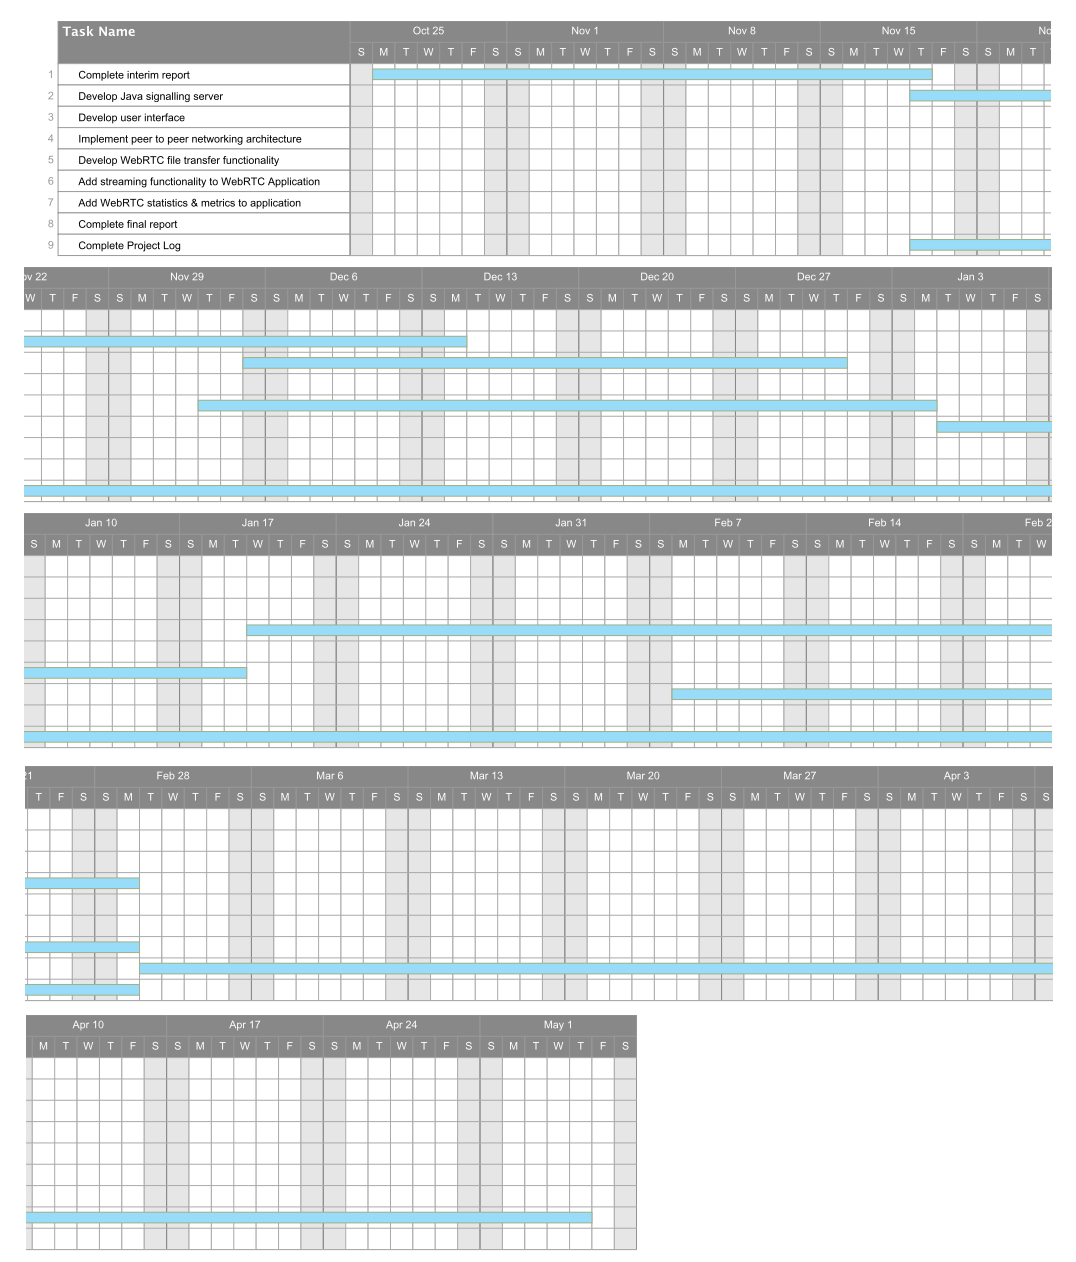
\includegraphics[scale=0.5]{ganttchart.png}
			\end{figure}
			\newpage	
			
			\subsection*{Risk Analysis}
				\todo{write more}
				\scalebox{0.6}{\begin{tabular}{@{}|l|l|l|l|l|@{}}
						\toprule
						\textbf{Risk}                                      & \textbf{Probability (1-5)} & \textbf{Impact (1-5)} & \textbf{Mitigation}                                                                                                  & \textbf{Contingency}                                                                            \\ \midrule
						Illness/Injury                                     & 4                          & 3                     & \begin{tabular}[c]{@{}l@{}}Reserve time for illness\\ Be hygienic\\ Eat healthy\\ Exercise\end{tabular}              & \begin{tabular}[c]{@{}l@{}}Allow time for recovery\\ Take medicine to aid recovery\end{tabular} \\ \midrule
						Inaccurate estimations                             & 3                          & 3                     & \begin{tabular}[c]{@{}l@{}}Be liberal with estimations\\ Reserve time for deliverables behind schedule\end{tabular}  & Adjust scope of project                                                                         \\ \midrule
						Data loss                                          & 1                          & 5                     & \begin{tabular}[c]{@{}l@{}}Use a version control system\\ Keep local backups\end{tabular}                            & Recover data from Git                                                                           \\ \midrule
						Uncommunicative stakeholder                        & 1                          & 3                     & Ensure regular meetings with stakeholder                                                                             &                                                                                                 \\ \midrule
						Stakeholder turnover                               & 1                          & 4                     & N/A (out of my control)                                                                                              & Get new stakeholders                                                                            \\ \midrule
						Project scope too large                            & 3                          & 4                     & \begin{tabular}[c]{@{}l@{}}Research enough to be certain in project scope\\ Be liberal with estimations\end{tabular} & Adjust scope of project                                                                         \\ \midrule
						Technologies too immature/insufficient for project & 2                          & 4                     & Research technologies beforehand                                                                                     & \begin{tabular}[c]{@{}l@{}}Find alternative technologies\\ Adjust scope of project\end{tabular} \\ \bottomrule
					\end{tabular}}
		
			\subsection*{Quality Analysis}
			The main measure of success will be the web application's performance in it's ability to transfer \& stream data between two peers. To track this, I will implement metrics using the WebRTC "getStats" statistics API, which allows for monitoring of peer connections. Further to this, once I have implemented a many-to-many peer-to-peer network, I will test the application with multiple peers in order to replicate load. The application will also be user tested to ensure it is user-friendly. The signalling server will be load tested in isolation to make certain it can handle multiple requests. 
			
	\section{Methodology}
		I chose to use an alternative methodology to the waterfall model because it lacks the ability to adapt to changes in a project deadline. Due to the way waterfall is structured into different phases that must be completed sequentially, often when changes such as new requirements occur, all these phases must be repeated in order to account for this. Iterative methodologies take an approach that can adapt to these changing requirements because they utilise short development cycles and focus on developing small modules of a product at one time, making it easier to revise a product if necessary. This is particular useful in my project as it is relatively experimental and the requirements of it may change regularly. 
		
		Thus, as a way of tracking the progression of my project, I plan to use an iterative and evolutionary methodology. This is used within software development as a way of incrementally developing applications through small cycles. Whilst it will be similar to scrum, it will not have the stricter framework surrounding it that requires a product owner and scrum master. This methodology will be relatively simple and based around a backlog of tasks from which a developer pulls from in a limited amount, normally 1 or 2 tasks at a time which will are then pushed through the development work flow.
		
		In my case, the work flow will be relatively simple:
		\begin{enumerate}
			\item To Do
			\item In Progress
			\item Code Review
			\item Manual Testing
			\item Done
		\end{enumerate}
		
		During the "In Progress" step of the work flow, I will use a test driven development (TDD) process in which tests are written first and then code is wrote to make the test work. However, I will be fairly lenient with this, only using this process on parts of the code that require stringent testing as writing unnecessary tests will take up development time. 
		
		\begin{figure}[h!]
			\caption{
				Test-Driven Development (TDD) Cycle
				\cite{TDD Diagram}
			}
			\centering
			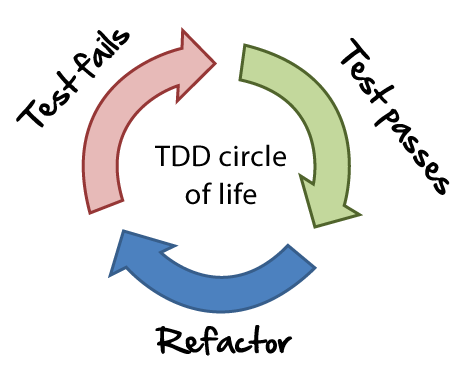
\includegraphics[scale=0.5]{tdd-circle-of-life.png}
		\end{figure}
		
		During the "Code Review" step, I plan to self-evaluate the task I have completed. On top of this, I will run static code analysis tools (such as FindBugs and PMD for Java) if the task is a coding task and use the code review section StackExchange to get second opinions. If it passes the code review step and it is possible to do so, I will black-box test the task from a user's perspective to see that it actually works as intended. Once every task forming a feature is completed, I will manually test the feature as a whole to see that each task has integrated together as planned.
		
		To visualise this workflow, I will use the open source web application "Kanboard" which I have hosted on an AWS EC2 Instance. This will allow me to keep track of progress throughout the duration of the project. To manage the actual changes made to the project files, I have utilised the version control system Git with a private GitHub repository containing my project.
		
	\begin{thebibliography}{20}
		\bibitem{CSA Top Threats}
		Cloud Security Alliance. (2013). The Notorious Nine Cloud Computing Top Threats in 2013. Available: https://downloads.cloudsecurityalliance.org/initiatives/top\_threats/The\_N\\otorious\_Nine\_Cloud\_Computing\_Top\_Threats\_in\_2013.pdf. Last accessed 09/11/2015.
		\bibitem{PRISM}
		Greenwald, Glenn; MacAskill, Ewen (June 6, 2013). "NSA Taps in to Internet Giants' Systems to Mine User Data". The Guardian.  Last accessed 05/11/2015.
		\bibitem{IPB Encryption}
		Andrew Griffin. (2015). Investigatory Powers Bill could allow Government to ban end-to-end encryption, technology powering iMessage and WhatsApp. Available: http://www.independent.co.uk/life-style/gadgets-and-tech/news/investigatory-powers-bill-could-allow-government-to-ban-end-to-end-encryption-technology-powering-a6725311.html. Last accessed 09/11/2015.
		\bibitem{WeTransfer Storage Time}
		WeTransfer. How long are my uploads available to download?. Available: https://wetransfer.zendesk.com/hc/en-us/articles/202603916-How-long-are-my-uploads-available-to-download-. Last accessed 05/11/2015.
		\bibitem{WeTransfer AWS Case Study}
		Amazon Web Services. WeTransfer Case Study. Available: https://aws.amazon.com/solutions/case-studies/wetransfer/. Last accessed 05/11/2015.
		\bibitem{Unstructured P2P Diagram}
		An Unstructured Peer-To-Peer Overlay Network. Available:
		http://www.hindawi.com/journals/jcnc/2012/485875/fig1/. Last Accessed 6 Nov. 2015.
		\bibitem{P2P overlay networks}
		Eng Keong Lua Crowcroft, J. ; Pias, M. ; Sharma, R. ; Lim, S.. (Second Quarter 2005). A survey and comparison of peer-to-peer overlay network schemes. Communications Surveys \& Tutorials, IEEE. 7 (2), 72 - 93.
		\bibitem{Hybrid P2P network}
		Yang, Beverly; Garcia-Molina, Hector (2001). Available: http://infolab.stanford.edu/~byang/pubs/hybridp2p\_long.pdf. Very Large Data Bases. Last Accessed 06/11/2015.
		\bibitem{P2P Security Issues}
		Schulzrinne, et al. (February 2010). Security in P2P Realtime Communications. Available: https://tools.ietf.org/html/rfc5765\#section-7.2. Last accessed 05/11/2015.
		\bibitem{WebRTC Security Study}
		N/A. A Study of WebRTC Security. Available: http://webrtc-security.github.io/\#4.3. Last accessed 05/11/2015.
		\bibitem{Google WebRTC Release}
		Harald Alvestrand. (2011). Google release of WebRTC source code. Available: http://lists.w3.org/Archives/Public/public-webrtc/2011May/0022.html. Last accessed 29/10/2015.
		\bibitem{W3C WebRTC Definition} 
		Adam Bergkvist, Daniel C. Burnett, Cullen Jennings, Anant Narayanan (until November 2012). (2011). WebRTC 1.0: Real-time Communication Between Browsers. Available: http://www.w3.org/TR/webrtc/. Last accessed 29/10/2015.
		\bibitem{WebRTC browser support}
		Available: http://iswebrtcreadyyet.com/. Last accessed 30/10/2015.
		\bibitem{Mozilla Web API}
		Mozilla Web API. Available: https://developer.mozilla.org/en-US/docs/Web/API. Last accessed 30/10/2015.
		\bibitem{JSEP}
		Justin Uberti. (2011). Javascript Session Establishment Protocol (JSEP). Available: https://lists.w3.org/Archives/Public/public-webrtc/2012Jan/att-0002/JavascriptSessionEstablishmentProtocol.pdf. Last accessed 11/11/2015.
		\bibitem{TDD Diagram}
		Available: http://www.agilenutshell.com/assets/test-driven-development/tdd-circle-of-life.png. Last accessed 09/11/2015.
	\end{thebibliography}

\end{document}          
